\documentclass[12pt]{article}

\usepackage{sectsty}
\usepackage{fullpage}
\usepackage{graphicx}

\sectionfont{\large}
\begin{document}\vspace{0.5in}
\begin{center}\begin{large}\textbf{Keshav Bihani}\end{large}\end{center}\textbf{\hrulefill}\\

\begin{tabular}{@{}p{4in}p{3in}}
Room No-A26 & {Phone:}+91-7753820605 \\
Dr. S RadhaKrishnan Hostel & {E-mail:}keshavbihani12@gmail.com\\
University of Allahabad \\
Allahabad\\
& 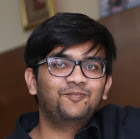
\includegraphics[scale=0.8]{keshav1.jpg}\\
\end{tabular}
\section*{Objective}
To utilize my technical skills towards developing systems that are smarter and can learn by itself; providing its users experience like never before.   
\section*{Education}
\begin{tabular}{|l|l|l|l|l|}
\hline
Degree & College/School & University & Passing Year & Pass Percentage\\
\hline
B. Tech & JKIAPT & Allahabad University & 2017 & 70 (till 5th sem)\\
\hline
High School & Delhi Public School & CBSE & 2012 & 90\\
\hline
Intermediate & Don Bosco School & ICSE & 2010 & 90\\
\hline
\end{tabular}

\section*{Projects}
\begin{itemize}
\item[$\bullet$]\textbf{Puzzle Solver Robot.}\\November 2015- Feb 2016\\Members: Raj Krishna, G. HarshaVardhan, Shantam Srivastava

This project was based on OpenCv and Python and implemented on Atmega 2560. It used basic image processing technique to sense an image and then solve the puzzle using the input image.
\item[$\bullet$]\textbf{Website for Alumni.}\\May 2015- July 2015\\Members: Varun Kumar Singh

This project was undertaken by two of us as a means to reach out to our almamater and build an interactive platform where the college and alumni could interact.
\item[$\bullet$]\textbf{Waste Segregating Robot.}\\October 2014-Jan 2015 \\Members: Raj Krishna, G. HarshaVardhan, Shantam Srivastava

This project was based on Atmega 2560 to segregate waste based on its size and colour.It did win the second position in eYRC competition amongst 52 other teams that participated.
\end{itemize}
\section*{Training and Internships}
\begin{enumerate}
\item Android Development.\\May 2014- July 2014. CMS Institute, Hyderabad.
\end{enumerate}
\section*{Technical Skills}
\begin{itemize}
\item[$\cdot$]Programming Languages
\begin{enumerate}
\item C
\item C++
\item Java
\item Python
\end{enumerate}
\item[$\cdot$]Knowledge of Data Structures and Algorithms.
\item[$\cdot$]Tools and Technologies Used
\begin{enumerate}
\item JSP
\item Atmel Studio
\item Android Studio
\item OpenCV.
\end{enumerate}
\end{itemize}
\begin{itemize}
\item[$\cdot$]
\end{itemize}
\section*{Soft Skills}
\begin{itemize}
\item[$\cdot$] Good Communication Skills with bilingual proficiency in English and Hindi.
\item[$\cdot$]Good presentation and management skills.
\item[$\cdot$]Great team player.
\item[$\cdot$]Affectionate and Optimistic. 
\end{itemize}
\section*{Extra-Curricular Activities}
\begin{itemize}
\item[$\cdot$]Robotics Competition.
\item[$\cdot$]Competitive Coding.
\end{itemize}
\section*{Co-Curricular Activities}
\begin{itemize}
\item[$\cdot$] Debate and JAM
\item[$\cdot$] Group Discussion 
\item[$\cdot$] Music
\item[$\cdot$] Playing Basketball 
\end{itemize}

\end{document}